\question{}

จงพิจารณากราฟที่กำหนดให้ต่อไปนี้

\begin{center}
    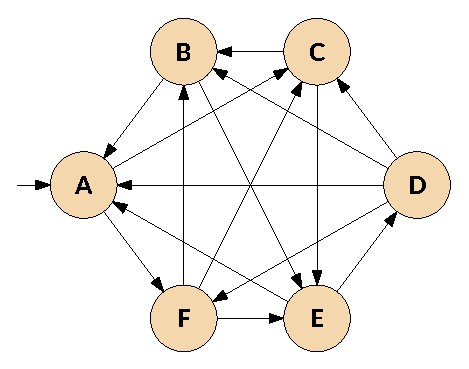
\includegraphics[]{figures/ponder_central_audition_infinitepath.eps}
\end{center}

ให้พิจารณากราฟที่กำหนดให้ เราจะเขียนโปรแกรมเพื่อเดิน (traverse) บนกราฟดังกล่าว โดยมีเงื่อนไขดังนี้
\begin{enumerate}
\item เราจะเริ่มต้นการเดินจากโหนด A
\item จากโหนดหนึ่ง ๆ เราจะเดินไปยังโหนดถัดไปเฉพาะโหนดที่มีลูกศรชี้ไปหาเสมอ

    หากมีลูกศรชี้ไปยังโหนดอื่น ๆ มากกว่า 1 โหนด ให้เลือกเดินไปโหนดถัดไป\uline{โหนดใดก็ได้}
    \uline{จากตัวเลือกนั้น ๆ} (เช่น จากโหนด B เราสามารถเดินไปยังโหนด A หรือ E โหนดใดก็ได้)
\item เราจะเดินบนกราฟนี้ไปเรื่อย ๆ ไม่มีหยุดอยู่กับที่ (เสมือนว่าโปรแกรมของเรามี infinite loop)
\end{enumerate}

\noindent
จากการเดินบนกราฟอย่างไม่สิ้นสุดตามคำอธิบายข้างต้น ข้อใดต่อไปนี้ถูกต้องบ้าง?

\begin{itemize}[label={$\square$}]
    \item \textbf{ประพจน์ P:} รับประกันว่าในการเดินดังกล่าว ``เราจะเดินพบโหนด A อนันต์ครั้ง'' 
        หรือไม่เช่นนั้น ``เราจะเดินพบโหนด D อนันต์ครั้ง''
    \item \textbf{ประพจน์ Q:} รับประกันว่าในการเดินดังกล่าว ``เราจะเดินพบโหนด B อนันต์ครั้ง'' 
        หรือไม่เช่นนั้น ``เราจะเดินพบโหนด E อนันต์ครั้ง''
    \item \textbf{ประพจน์ R:} รับประกันว่าในการเดินดังกล่าว ``เราจะเดินพบโหนด C อนันต์ครั้ง'' 
        หรือไม่เช่นนั้น ``เราจะเดินพบโหนด F อนันต์ครั้ง''
\end{itemize}
